


\section{Sampling distribution of OLS}
Note that the OLS estimate that we are getting is a random variable - the estimate we get is different depending on which sample we work with. This is why we can discuss the distributional properties - mean and variance, in particular - of the OLS. 
\begin{itemize}
\item $\hat{\beta}_1$: Recall that we can write
\[
\hat{\beta}_1= \frac{\sum_{i=1}^n(X_i-\bar{X})(Y_i-\bar{Y})}{\sum_{i=1}^n(X_i-\bar{X})^2}
\]
Now, replace $Y_i$ an $\bar{Y}$ with 
\[
Y_i =\beta_0 + \beta X_i + u_i, \ \bar{Y} = \beta_0 + \beta_1\bar{X} + \bar{u},
\]
which allows us to write 
\[
(Y_i-\bar{Y}) = (\beta_1(X_i-\bar{X})+(u_i-\bar{u}))
\]
and get
\[
\hat{\beta}_1=\beta_1+  \frac{\sum_{i=1}^n(X_i-\bar{X})(u_i-\bar{u})}{\sum_{i=1}^n(X_i-\bar{X})^2}
\]
We are now ready to discuss the distributional properties
\begin{itemize}
\item $E[\hat{\beta}_1]$: It can be written as
\[
\begin{aligned}
E[\hat{\beta}_1]& = E\left[\beta_1+  \frac{\sum_{i=1}^n(X_i-\bar{X})(u_i-\bar{u})}{\sum_{i=1}^n(X_i-\bar{X})^2}\right]\\
&=\beta_1+ E\left[\frac{\sum_{i=1}^n(X_i-\bar{X})(u_i-\bar{u})}{\sum_{i=1}^n(X_i-\bar{X})^2}\right]
\end{aligned}
\]
Note that the $\sum_{i=1}^n(X_i-\bar{X})(u_i-\bar{u})$ can be written to something simpler. This is equal to
\[
\sum_{i=1}^n(X_i-\bar{X})(u_i-\bar{u})=\sum_{i=1}^nX_iu_i-\bar{u}\sum_{i=1}^n X_i+\bar{X}\sum_{i=1}^nu_i+n\bar{X}\bar{u}
\]
Since $\bar{X}$ is a sample mean of $X$, $\sum_{i=1}^nX_i=n\bar{X}$. The assumption that conditional mean is zero and $(X_i, u_i)$ are uncorrelated means that the term on the left hand side is zero. Therefore, IF THE CLASSICAL ASSUMPTIONS ARE VALID, $E[\hat{\beta}_1]=\beta_1$.
\item $var[\hat{\beta}_1]$: We use the definition of the variances and the fact that the expected value of $\hat{\beta}_1$ is unbiased (at least for now) to get
\[
\begin{aligned}
var(\hat{\beta}_1)&=E\left[\left(\hat{\beta}_1-E[\hat{\beta}_1]\right)^2\right] \\
&=E\left[\left(\hat{\beta}_1-{\beta}_1\right)^2\right]\\
&=E\left[\left( \frac{\sum_{i=1}^n(X_i-\bar{X})(u_i-\bar{u})}{\sum_{i=1}^n(X_i-\bar{X})^2} \right)^2\right]\\
&=E\left[\left(  \frac{(X_1-\bar{X})(u_1-\bar{u})}{\sum_{i=1}^n(X_i-\bar{X})^2}+...+\frac{(X_n-\bar{X})(u_n-\bar{u})}{\sum_{i=1}^n(X_i-\bar{X})^2} \right)^2\right]\\
\end{aligned}
\]
At the moment, we are assuming homoskedasticity and no autocorrelation (A3, A4). Since $X_i$ is from the data and $u_i$ is a random error term, we can take all the $X_i$ terms in and keep the $u_i$ terms in the expectation to get (i.i.d assumption is also useful here)
\[
\begin{aligned}
var(\hat{\beta}_1)&=\frac{\sum_{i=1}^n(X_i-\bar{X})^2E[(u_i-\bar{u})^2]}{[\sum_{i=1}^n(X_i-\bar{X})^2]^2}\\
&=\frac{\sum_{i=1}^n(X_i-\bar{X})^2\sigma_u^2}{[\sum_{i=1}^n(X_i-\bar{X})^2]^2} \ (\because E[(u_i-\bar{u})^2=var(u_i))\\
&=\sigma_u^2\frac{\sum_{i=1}^n(X_i-\bar{X})^2}{[\sum_{i=1}^n(X_i-\bar{X})^2]^2} =\frac{\sigma_u^2}{\sum_{i=1}^n(X_i-\bar{X})^2}
\end{aligned}
\]
Note that  to decrease the variance in the estimates, the variance of the error should be small relative to the variation in the $X_i$. 
\end{itemize}
At the end of the day, we can say the following about the distribution of our $\hat{\beta}_1$ estimator and use this to test our hypothesis
\[
\hat{\beta}_1 \sim N\left(\beta_1, \frac{\sigma_u^2}{\sum_{i=1}^n(X_i-\bar{X})^2}\right)
\]
\item $\hat{\beta}_0$: The formula for $\hat{\beta}_0$ is $\bar{Y}-\hat{\beta}_1\bar{X}$. By changing $\bar{Y}$, we can get
\[
\begin{aligned}
\hat{\beta}_0&=(\beta_0+\beta_1\bar{X}+\bar{u})-\hat{\beta}_1\bar{X}\\
&=\beta_0+(\beta_1-\hat{\beta}_1)\bar{X}+\bar{u}
\end{aligned}
\]
Then we can say the following about the sampling distribution
\begin{itemize}
\item $E[\hat{\beta}_0]$: We can write
\[
E[\hat{\beta}_0]=\beta_0+E[(\beta_1-\hat{\beta}_1)\bar{X}]+E[\bar{u}]=\beta_0
\]
since $\hat{\beta}_1$ is unbiased and conditional expectation of $u_i$ is zero. Thus, under our current assumptions, $\hat{\beta}_0$ is unbiased. 
\item $var[\hat{\beta}_0]$: Using the definition of the variance, we can write \[
\begin{aligned}
var(\hat{\beta}_0)&=E\left[\left(\hat{\beta}_0-E[\hat{\beta}_0]\right)^2\right] \\
&=E\left[\left(\hat{\beta}_0-{\beta}_0\right)^2\right]\\
&=E\left[\left( (\beta_1-\hat{\beta}_1)\bar{X}+\bar{u}\right)^2\right]\\
&=\bar{X}^2E\left[\left(\beta_1-\hat{\beta}_1 \right)^2\right]+ 2\bar{X}E\left[\left(\beta_1-\hat{\beta}_1 \right)\bar{u}\right] + E[\bar{u}^2]
\end{aligned}
\]
Under the assumption (A2), we can ignore the middle term as this is zero. The rest of the terms are $\bar{X}^2 var(\hat{\beta}_1)$ and $\frac{\sigma_u^2}{n}$. the final result is
\[
var(\hat{\beta}_0)=\frac{\sigma_u^2\bar{X}^2}{\sum_{i=1}^n(X_i-\bar{X})^2}+\frac{\sigma_u^2}{n}= \frac{\sigma_u^2}{n}\frac{\sum_{i=1}^nX_i^2}{\sum_{i=1}^n(X_i-\bar{X})^2}
\]
\end{itemize}
So we can write 
\[
\hat{\beta}_0 \sim N\left(\beta_0, \frac{\sigma_u^2}{n}\frac{\sum_{i=1}^nX_i^2}{\sum_{i=1}^n(X_i-\bar{X})^2}\right)
\]
\end{itemize}

\section{Hypothesis Tests}
We now have a sampling distribution for our OLS estimator. This now allows us to create a test statistic for the hypothesis test. In this note, we will talk about testing for the slope coefficient $\beta_1$. The idea is similar for our intercept $\beta_0$ and even if we have multiple $X_i$ variables. 
\begin{itemize}
\item\textbf{Test statistics} We know that the sampling distribution for $\hat{\beta}_1$ is
\[
\hat{\beta}_1 \sim N\left(\beta_1, \frac{\sigma_u^2}{\sum_{i=1}^n(X_i-\bar{X})^2}\right)
\]
To make the discussion simple, I now write $var(\hat{\beta}_1)=\frac{\sigma_u^2}{\sum_{i=1}^n(X_i-\bar{X})^2}$. There are two ways we go about this. One is where we know that actual value of $var(\hat{\beta}_1)$, through knowing $var(u_i)=\sigma_u$. The other case is where we do not know the exact value of $\sigma_u$ and are forced to estimate $var(u_i)$.
\item[$\to$] \textit{If we know $\sigma_u$}: This is a relatively easy case. Since the $\hat{\beta}_1$ takes a normal distribution, we can ``standardize" it to get the test statistic and the distribution for it. To do so, we simply subtract the mean from the estimate and divide the term by the standard deviation. That gets us
\[
\frac{\hat{\beta}_1-\beta_1}{\sqrt{var(\hat{\beta}_1)}}\sim N(0,1)
\]
Typically, the hypothesis test we use is (this is the default for the output tables in STATA)
\[
H_0: \beta_1=0 \ \ \text{vs} \ \ H_1: \beta_1\neq0
\]
Then, the test statistic becomes 
\[
t=\frac{\hat{\beta}_1}{\sqrt{var(\hat{\beta}_1)}}
\]
and you get to compare against the critical values that comes from the standard normal distribution. The critical values you use is determined by the significance level (5\% or 1\%), and the type of test you run (one vs two-tails).
\item[$\to$] \textit{If we don't know $\sigma_u$}: We are a bit unlucky in this case, but not by far. The difference is that you need to have an estimate for $var(\hat{\beta}_1)$ due to not knowing $\sigma_u$. The test statistics and its distribution is
\[
\frac{\hat{\beta}_1-\beta_1}{\sqrt{\widehat{var(\hat{\beta}_1)}}}\sim t_{n-2}
\]
where $\widehat{var(\hat{\beta}_1)}$ is the estimate for the variance and $t_{n-2}$ is a t-distribution with $n-2$ degrees of freedom. The degrees of freedom is determined by the number of observations, where 2 is subtracted because we are estimating $\beta_0$ and $\beta_1$ in the process. (\textit{Spoiler: In the multiple variable case with a constant and $k$ control variables, the degree of freedom is $n-k-1$}). Other than these differences, the idea that you need to compare with the appropriate critical value still carries over. \par\medskip
One comforting fact is that when $n$ is very large, t-distribution becomes very similar to the normal distribution. so the process of finding critical values are identical to the previous case.
\item \textbf{Confidence interval}: A 95\% confidence interval is a range of numbers that form a random interval that has a 95\% chance of including a (nonrandom) true value of a parameter. This can be obtained by inverting the rejection region that we have used in the critical value approach. \par\medskip
To make this simple, let's use a two-sided test  with 5\% significance level. as an example. Typically, the critical values are $\pm1.96$. We can tell that 
\[
\Pr\left(-1.96\leq \frac{\hat{\beta}_1-\beta_1}{\sqrt{var(\hat{\beta}_1)}} \leq1.96\right)=0.95
\]
We can switch around some terms to get $\beta_1$ in the middle, as a result
\[
\Pr\left(\hat{\beta}_1-1.96\times\sqrt{var(\hat{\beta}_1)} \leq \beta_1 \leq\hat{\beta}_1+1.96\times\sqrt{var(\hat{\beta}_1)}\right)=0.95
\]
In this way, we can find the upper and lower bounds of the confidence intervals. If they encompass the null test value - 0, for instance - then we cannot reject the null hypothesis. Otherwise, we can reject the null. 
\end{itemize}

\section{Bivariate Independent Variables}

Throughout the course, we have assumed that the independent variable $X_i$ can take any values. However, we may be interested in whether there is a difference in outcome due to affiliation to a certain group (nationality, for instance). Most of these can only be represented by either being part of the group, or not being part of the group. To analyze these cases, we need to understand what \textbf{dummy variable} is (some textbooks call it indicator variables). If $X_i$ is a dummy variable, it is mathematically defined as
\[
X_i = \begin{cases} 1 & \text{if $i$ belongs in group $X$} \\  0 & \text{if otherwise} \\ \end{cases}
\]
\par\medskip
While the OLS methods we have learned so far can be applied, there is a subtle change when it comes to interpretation. Now $\hat{\beta}_1$ is no longer the slope anymore. However, using conditional expectations make the interpretation much clearer.
\[
\begin{aligned}
E[Y_i |X_i=0]=& \beta_0\\
E[Y_i |X_i=1]=& \beta_1+\beta_0\\
\end{aligned}
\]
Therefore, $\beta_1$ is then the difference in mean between $X_i=1$ and $X_i=0$ at the population level. When you are estimating $\hat{\beta}_1$, you are estimating for group differences in expected values. This can be graphically expressed as a ``jump" at the point where $X_i=1$. \par\medskip
Dummy variables can be implemented in STATA in these methods. One is to use \texttt{generate} and \texttt{replace} command. Start by typing in \texttt{generate smallsize =0}. Then define conditions that would make smallsize variable 1 and replace by using \texttt{replace smallsize =1 if str<19}. The other is to use \texttt{tabulate} command. This is particularly useful if you are making a dummy variable straight out of a non-numerical variable. Type in \texttt{tabulate variable, generate(new dummy name)}. Then this command generates dummy variables for each category recorded in the original variable. If there were 10 types of answers in the original variable, then 10 new variables will be generated. \par\medskip 
\section{Heteroskedasticity}
We have assumed that the variance of the error term $var(u_i)$ is not a function of $X_i$. However, this assumption may not hold. In case where they do not hold, we can observe that the variance estimated under homoskedasticity assumption is (usually) underestimated. The graph on the left side is for the observations following the homoskedasticity assumption, while the one on the right does not follow homoskedasticity assumption.
\begin{figure}[H]
\centering
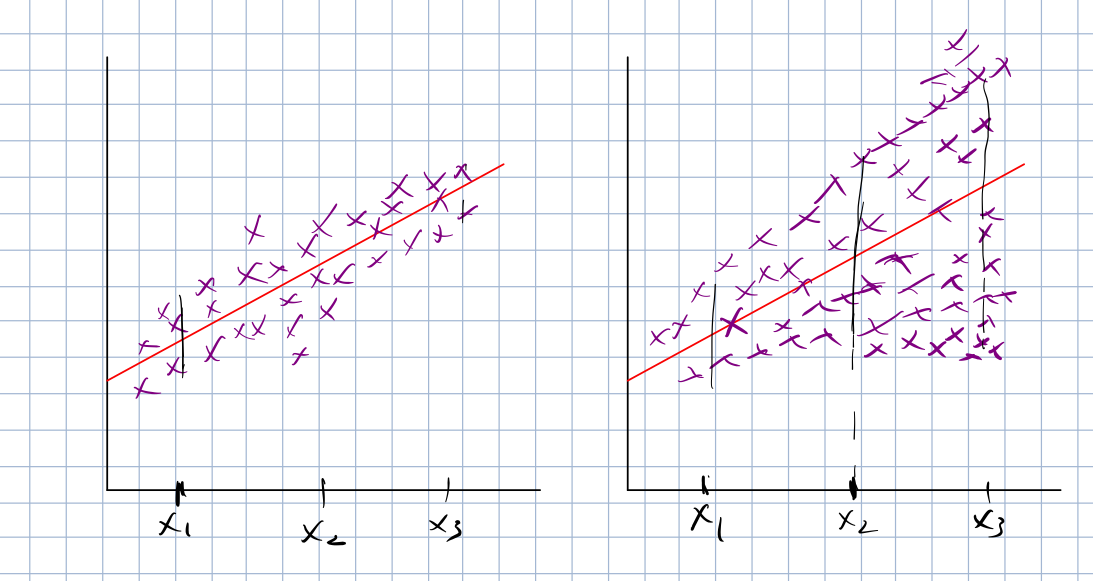
\includegraphics[width=0.55\textwidth]{hetero.png}
\end{figure}
\par\medskip
From the figure, we can see that the variance of the error term changes with $X_i$. In such case, standard errors of our estimators must take this into account. Running two versions of the regression in STATA would help. The homoskedastic version could be obtained by \texttt{regress y x}, while the heteroskedastic version requires \texttt{regress y x, vce(robust)} or \texttt{regress y x, robust}.  Below, I regressed the codes from the previous recitation for comparison. \par\medskip
\begin{figure}[H]
\centering
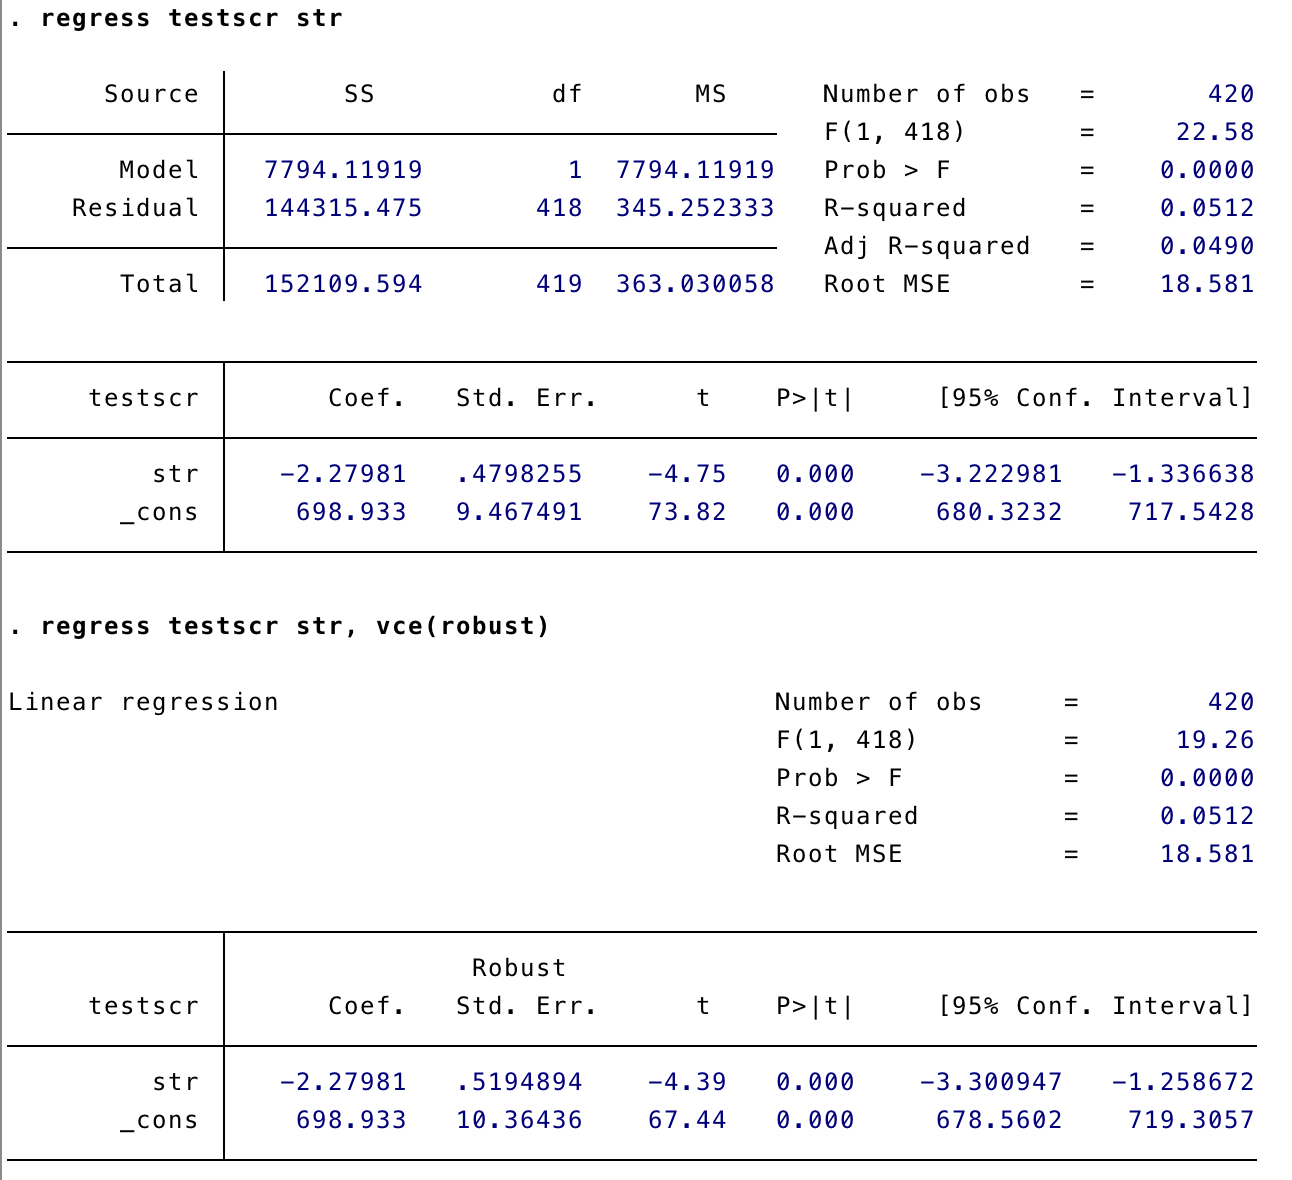
\includegraphics[width=0.7\textwidth]{heterovhomo.png}
\end{figure}
There are two takeaways from the picture
\begin{itemize}
\item \textbf{The variance rises (usually) in the heteroskedastic regression.} In other words, when we keep homoskedasticity assumption in cases where we should not do so, we end up rejecting null hypothesis that should not be rejected.
\item \textbf{The coefficients are unchanged.} When calculating the values for the estimators, we did not rely on the homoskedasticity assumption. Therefore, the coefficients are unaffected. In other words, the estimates are still unbiased.
\end{itemize}

\section{Omitted variable bias}
So far, we have assumed that the number of our independent variable (other than the intercept term) is just one. We now extend our discussion to include more than one independent variable. 
\par\medskip
Before, we regressed whether test score is affected by the size of the classrooms. For every other factor that could affect the test score, we did not include them. However, one might guess that the higher the average income of a county, the higher the test score. Assume that this does affect the test score. Moreover, it is quite likely that richer neighborhoods can afford better school infrastructure and educational quality, leading to smaller size of classrooms. If this is the case, then the model that we have at the moment - without average income of the county - is not capturing the effect of classroom size on test score accurately. \par\medskip 
This is a case of an \textbf{omitted variable bias}. If there is an omitted variable bias, then the estimate we have of the effect of $X_i$ on $Y_i$ is not accurate and thus biased. One formal way to express this issue is as follows: Suppose that the true population regression model and the sample regression model is 
\[
\begin{aligned}
\text{True: }& Y_i = \beta_0 + \beta_1 X_i + \beta_2 Z_i+u_i\\
\text{Mistake: }& Y_i = \beta_0 + \beta_1 X_i + u_i^*\\
\text{Sample: }& Y_i = \hat{\beta}_0 + \hat{\beta}_1 X_i+ \hat{u}_i\\
\end{aligned}
\]
Suppose you run an OLS regression without $Z_i$. As discussed in previous lectures, the OLS estimator for $\beta_1$ can be calculated as $\frac{\sum_{i=1}^n(X_i-\bar{X})(Y_i-\bar{Y})}{\sum_{i=1}^n(X_i-\bar{X})^2}$. However, if you include the $(Y_i-\bar{Y})$ from the true regression model, the OLS estimator now becomes
\[
\begin{aligned}
\frac{\sum_{i=1}^n(X_i-\bar{X})(Y_i-\bar{Y})}{\sum_{i=1}^n(X_i-\bar{X})^2} =& \frac{\sum_{i=1}^n(X_i-\bar{X})(\beta_1(X_i-\bar{X})+\beta_2(Z_i-\bar{Z})+(u_i-\bar{u}))}{\sum_{i=1}^n(X_i-\bar{X})^2}\\
=& \beta_1 + \beta_2\frac{\sum_{i=1}^n(X_i-\bar{X})(Z_i-\bar{Z})}{\sum_{i=1}^n(X_i-\bar{X})^2}+\frac{\sum_{i=1}^n(X_i-\bar{X})(u_i-\bar{u})}{\sum_{i=1}^n(X_i-\bar{X})^2}\\
\end{aligned}
\]
Notice the term $\beta_2\frac{\sum_{i=1}^n(X_i-\bar{X})(Z_i-\bar{Z})}{\sum_{i=1}^n(X_i-\bar{X})^2}$. If $\beta_2 \neq0$ and $\frac{\sum_{i=1}^n(X_i-\bar{X})(Z_i-\bar{Z})}{\sum_{i=1}^n(X_i-\bar{X})^2}\neq 0$, then the mean of $\hat{\beta}_1$ is not guaranteed to be $\beta_1$. This is the reason why omitted variable bias causes inaccurate estimate of $\hat{\beta}_1$. These happen when both of the following cases hold
\begin{itemize}
\item \underline{$Z$ should explain $Y$}: If the slope coefficient of $Z$ is nonzero, then the $Z$ variable is part of the error term if we forget to include them
\item \underline{$Z$ is correlated with $X$}: If $cov(X,Z)\neq0$ and the regression residual $\hat{u}$ is correlated with $Z$, the independent variable is now correlated with $\hat{u}$, which leads to violation of the assumption that independent variable and the residual are not correlated.
\end{itemize} \par\medskip
If both conditions hold, the estimated effect of $X_1$, which is $\hat{\beta}_1$ is not unbiased and is inconsistent. This leads to the result where $E[u^*_i|X_i]=0$ assumption does not hold. There is a formal way to show this with equations.
\par\medskip
With the above formula, we can even determine the direction of the omitted variable bias - whether an estimate is biased downward or upward. The direction of the bias is determined by the sign of the $\beta_2\frac{\sum_{i=1}^n(X_i-\bar{X})(Z_i-\bar{Z})}{\sum_{i=1}^n(X_i-\bar{X})^2}$ term. If this term is positive, then the estimated $\hat{\beta}_1$ becomes larger than the true $\beta_1$. Thus, the estimate is said to be \textbf{overestimated}. If otherwise, $\hat{\beta}_1$ becomes smaller than the true $\beta_1$, making $\hat{\beta}_1$ \textbf{underestimated}.
\par\medskip
In order to address this issue, we can simply include the $Z$ variable if we have the data for it. Another way is to conduct an ideal randomized controlled experiment that randomly assigns \textit{str} to all students. If none of the two are feasible, we should find another variable that can be a proxy to $Z$ - they have to be related to the $X$ variable and is uncorrelated with the errors - which is the Instrumental Variable method. \par\medskip

\section{Multivariate Regression}
\textbf{Multivariate Regression} is simply a regression that involves more than one independent variables. The technicalities involved do not change drastically compared to the univariate regression. However, one should interpret the coefficients cautiously. Suppose that the regression is
\[
Y_i = \beta_0 + \beta_1 X_i + \beta_2 Z_i+u_i
\]
and the variable of interest is $X_i$. To see the impact of $X_i$ and $Y_i$, one needs to take (partial) derivatives on $Y_i$ with respect to $X_i$. This leads to
\[
\beta_1 = \frac{\partial Y_i}{\partial X_i}
\]
In words, $\beta_1$ captures how much $Y_i$ changes with respect to $X_i$ \emph{holding other variables constant} (ceteris paribus). If you do not hold other variables ($Z_i$ in this case) fixed, the change will not exactly be $\beta_1$ (it could be more or less). The statement \emph{holding other variables constant} is crucial in interpreting the $\beta_1$ coefficient.
\par\medskip

%%%%%%%%%%%%%%%%%%



